\section{Introduction}
\label{sec:intro}

When speaking about mobile devices and wearables, it might not be exactly clear which kind of hardware we are talking about.

Mobile devices are smartphones or tablets in this context. Most of the currently available mobile devices offer capabilities that could only be expected from desktop PCs a few years ago.

Wearables can be described as technology gadgets that one can wear on the body, e.g. around the wrist.
Usually they are loaded with sensors and can be connected to an other mobile device via Bluetooth.
The most commonly used wearables are smartwatches and fitness trackers, but the technology can also be found in clothing or jewelery.

\subsection{Motivation}
\label{sec:intro:motivation}

The data produced by sensors on wearables can be valuable for multiple use cases, for example:
\begin{itemize}[noitemsep]
	\item \textbf{Activity feedback}:
	A big selling point for wearables is the ability to track fitness activities in order to improve the health of the person wearing them.
	Of course this tracking works by analyzing sensor data, e.g. to count the steps or track the heart rate.
	\item \textbf{Event triggers}:
	Many wearables lack large user interfaces - in order to interact with them, one can use gestures.
	A smartwatch can turn its screen on if a user raises the wrist, but in the background a gesture detection system requires access to the device orientation and acceleration.
\end{itemize}

While some wearables can work as stand-alone devices, they usually depend on connected mobile devices to some extend.
That is because the available space for hardware components is very limited, leading to a lower battery and CPU\footnote{Central processing unit} power.
However, the device sensors on wearables can produce a large amount of data every second.
This data may needs to be pre-processed, analyzed or persisted - all of which requires a lot of processing power and will drain the device battery.
Thus, heavy work loads like these should be done on a connected mobile device and require a performant way to transfer data.

\subsection{Project Scope}
\label{sec:intro:scope}
The goal of our Bachelor project ``Passwords are Obsolete - Seamless authentication using wearables and mobile devices.'' was to authenticate a user by utilizing only data from devices that the user already owns.
We opted for training classifiers to analyze how a user performs certain activities and to distinguish between behavior patterns. These classifiers take raw sensor data or extracted features and perform different machine learning methods.

\begin{figure}[H]
	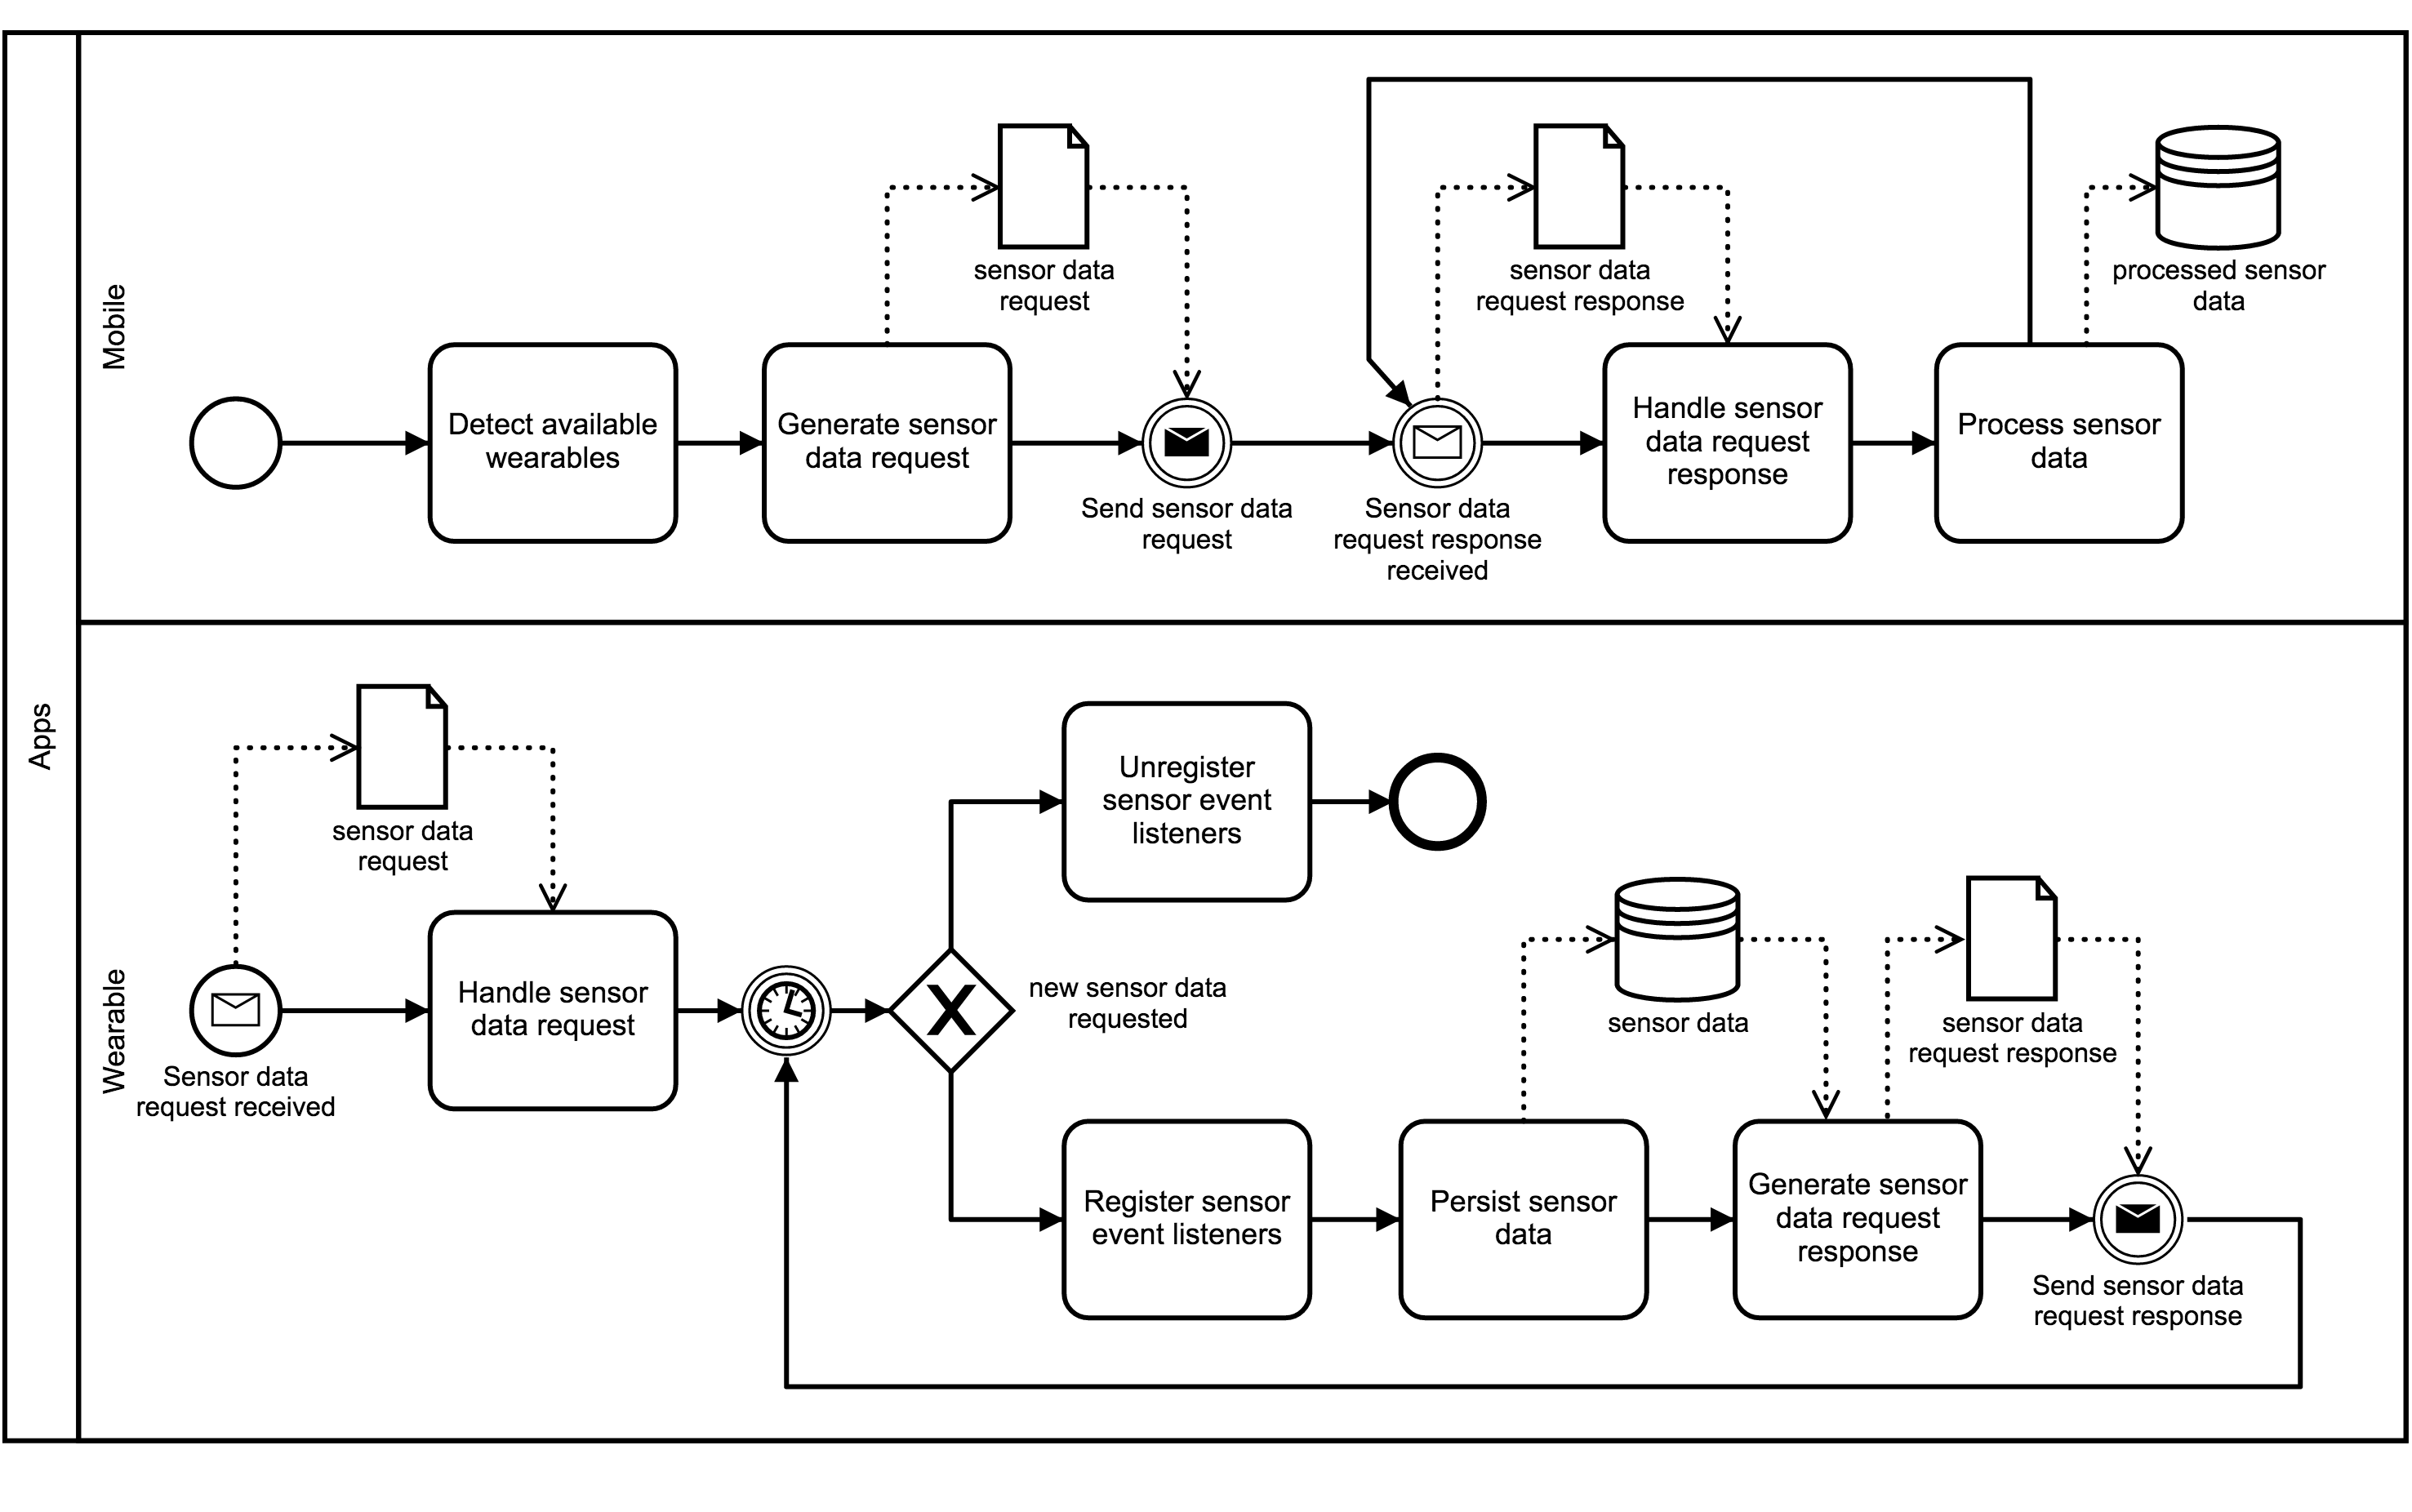
\includegraphics[width=\linewidth]{diagrams/apps.png}
	\caption[Caption for bpmn]{Trust level approach}
	\label{fig:diagrams:approach}
\end{figure}

Our unsupervised learning approach required that a wearable can exchange data with a mobile device in a performant jet battery friendly way while keeping the delay in an acceptable range.
This requirement is the topic of this thesis, structured as described below:

We will start with \textbf{Related Work} (\ref{sec:relatedwork}), where we briefly mention similar projects and papers related to this topic.
After that, we will let you know why we decided to develop for the Android platform in the \textbf{Devices} section (\ref{sec:devices}).
In \textbf{Concept} (\ref{sec:concept}), we will explain how the basic app setup on mobile and wearable devices needs to look like.
Actual code samples will be part of the \textbf{Implementation} section (\ref{sec:implementation}), where we provide detailed examples for every required functionality.
In \textbf{Evaluation} (\ref{sec:evaluation}) we will verify our solution using benchmarks and comparisons.
Possible improvements will be described in \textbf{Future work} (\ref{sec:futurework}).
Finally, \textbf{Conclusion} (\ref{sec:conclusion}) will wrap up our work.


\clearpage